\documentclass{article} %选择文档类型,我们如果是做期末大作业的话选article就可以了

%正如c++需要import库来实现各种各样的功能,Latex也需要调用宏包来实现各种各样的功能
\usepackage{amsmath}  %调用公式宏包
\usepackage{graphicx} %调用插图宏包
\usepackage{ctex}     %调用中文宏包
\usepackage{listings}
\usepackage{fancyhdr} %调用页眉页脚宏包
\usepackage{listings}
\usepackage{xcolor}
\usepackage[table]{xcolor}
\usepackage{amsmath}
\usepackage{subfigure}
\usepackage{graphicx}
\usepackage{booktabs}
\usepackage{float}
\usepackage{hyperref}
\usepackage{placeins} %避免图片乱跑,要在图片后面加上\FloatBarrier
\pagestyle{fancy} %设置页面风格为fancy
\setCJKmainfont{FandolSong}
% \lstset{
%   language=R,
%   frame=single,
%   framesep=5pt,
%   framerule=0.5pt,
%   backgroundcolor=\color{white},
%   basicstyle=\ttfamily\small,
%   keywordstyle=\color{blue},
%   stringstyle=\color{purple},
%   commentstyle=\color{green!70!black},
%   rulecolor=\color{black},
%   breaklines=true,
%   postbreak=\mbox{\textcolor{red}{$\hookrightarrow$}\space},
%   showstringspaces=false
% }

\lstset{
  language=R, % 设置语言
  basicstyle=\small\ttfamily, % 设置字体族
  breaklines=true, % 自动换行
  keywordstyle=\bfseries\color{blue}, % 设置关键字为粗体,颜色为 NavyBlue
  morekeywords={}, % 设置更多的关键字,用逗号分隔
  emph={self}, % 指定强调词
  emphstyle=\bfseries\color{Rhodamine}, % 强调词样式设置
  commentstyle=\itshape\color{black!50!white}, % 设置注释样式,斜体,浅灰色
  stringstyle=\bfseries\color{blue}, % 设置字符串样式
  breaklines=true,
  columns=fullflexible,
%   numbers=left, % 显示行号在左边
%   numbersep=2em, % 设置行号的具体位置
  numberstyle=\footnotesize, % 缩小行号
%   frame=single, % 边框
  framesep=1em, % 设置代码与边框的距离
  backgroundcolor=\color{gray!5} % 设置背景颜色为浅灰色
}
%清除默认的页眉和页脚
\fancyhf{} 

%设置页眉内容
\lhead{大数据分析2101} %左侧页眉内容
\rhead{时间序列分析项目报告} %右侧页眉内容

\fancyfoot[C]{第 \thepage 页} % 右侧页脚设置为页码
%\begin{document}这句话之前是导言区,这句话以后就开始写正文了
%可以把导言区理解为int main()函数之前的内容,而正文就是int main()主函数的部分了
\begin{document}




%标题封面部分
\begin{titlepage}
    \begin{center}
        \begin{figure}[H]
            \centering
            
\includegraphics[width=0.7\textwidth]{./pic/校名.pdf}
          \end{figure} 
          \huge \textbf{时间序列分析项目报告} \\ 
          \large \textbf{2023/2024(2)}
          \begin{figure}[H]
            \centering
            
\includegraphics[width=0.3\textwidth]{./pic/校徽.pdf}
          \end{figure}

          \vspace{0.5cm}

          \large 课题名称\hspace{0.8cm}\underline{\makebox[5.5cm]{苹果公司股票的时间序列分析}} \\
          \vspace{0.2cm}
            \large 小组成员1\hspace{0.5cm}\underline{\makebox[5.5cm]{Jiawei Wen(202103151422)}} \\
            \vspace{0.2cm}
            \large 小组成员2\hspace{0.5cm}\underline{\makebox[5.5cm]{Wangzi Chen(202103150503)}} \\
            \vspace{0.2cm}
            \large 小组成员3\hspace{0.5cm}\underline{\makebox[5.5cm]{Haifan Zhou(202105120127)}} \\  
            \vspace{0.2cm} 
            \large 代码编写\hspace{0.9cm}\underline{\makebox[5.5cm]{Wen, Chen, Zhou}} \\  
            \vspace{0.2cm} 
            \large 小组报告\hspace{0.9cm}\underline{\makebox[5.5cm]{Wen, Chen, Zhou}} \\  
            \vspace{0.2cm} 
            \large PPT制作\hspace{0.9cm}\underline{\makebox[5.5cm]{Wen, Chen, Zhou}} \\  
            \vspace{0.2cm}
            \large PPT汇报\hspace{0.9cm}\underline{\makebox[5.5cm]{Wangzi Chen}} \\  
            \vspace{2.5cm}
            \Large \heiti{理学院}
        \end{center}
\end{titlepage}

\clearpage % 避免标题页和正文之间的重叠


\tableofcontents
\listoffigures
\listoftables
\newpage

%分章节的示例,Latex会自动帮忙给标题编号
\section{背景介绍}

在当今全球化金融市场背景下,股票价格波动性的研究已成为金融学领域的重要议题。随着市场复杂度与互联性的增强,股票价格的波动不仅受到宏观经济环境、企业财务表现、投资者情绪、政策调整及全球事件等多元因素的影响,更呈现出显著的非线性与随机性特征。这一复杂动态网络要求我们采用更加精细与系统的方法来解析其中的内在规律,以期提升投资决策的准确性与效率。

时间序列分析,作为一种强大的统计工具满足了这一需求。它通过对一系列按时间顺序排列的数据点进行分析,揭示出隐藏于数据背后的模式与趋势。在金融领域,尤其是针对股票价格的研究中,时间序列被定义为一连串在特定时间点上观测到的随机变量\(X(t)\)的样本实现\(\{X_{t_1}, X_{t_2},\cdots, X_{t_N}\}\),其中\(t_1, t_2, \cdots, t_N\)代表了离散的时间点。这种离散特性与股票市场的交易特性不谋而合,使得时间序列分析成为剖析股票价格波动的理想方法。

苹果公司,作为全球市值领先的科技巨头之一,其产品与服务覆盖了消费电子、软件开发、数字内容等多个关键领域,拥有庞大的用户基础与品牌忠诚度。因为苹果公司在全球科技产业中的独特地位与深远影响力,本文将聚焦于苹果公司股票价格的时间序列分析。

\begin{figure}[h] % 开始一个浮动体环境,[h]指定为 here(这里)位置
	\centering % 图片居中
	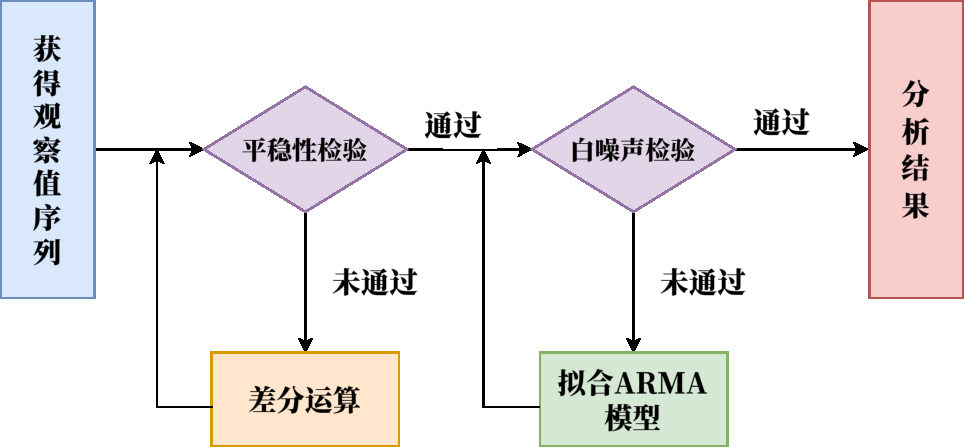
\includegraphics[width=\textwidth]{pic/ARIMA_new.pdf} % 插入宽度为文本宽度一半的图片
	\caption{ARIMA建模步骤} % 图片标题
	\label{} % 图片标签,用于引用
\end{figure}
\FloatBarrier

\section{原始数据分析}

\subsection{时序图}
在本节中,我们着手于对苹果公司股票价格数据进行直观的视觉呈现,旨在揭示其长期走势特征及潜在的时间序列属性。为此,我们精心构建了股票价格的时序图,这一图表生动地描绘了苹果公司股价自1990年2月1日至2011年10月14日间的演变轨迹(代码片段如列表所示)。

\begin{lstlisting}
    report <- read.csv("~\\Desktop\\大三下\\时间序列分析\\课程设计\\report.csv")
    report = ts(report)
    Start <- as.Date('1990-2-1')
    End <- as.Date('2011-10-14')
    dt <- seq(from = Start, to = End, by = 1)
    plot(report, main = 'Apple 股票趋势', xlab = '时间', ylab = '股价', type = 'o')
\end{lstlisting}

\begin{figure}[h] % 开始一个浮动体环境,[h]指定为 here(这里)位置
	\centering % 图片居中
	%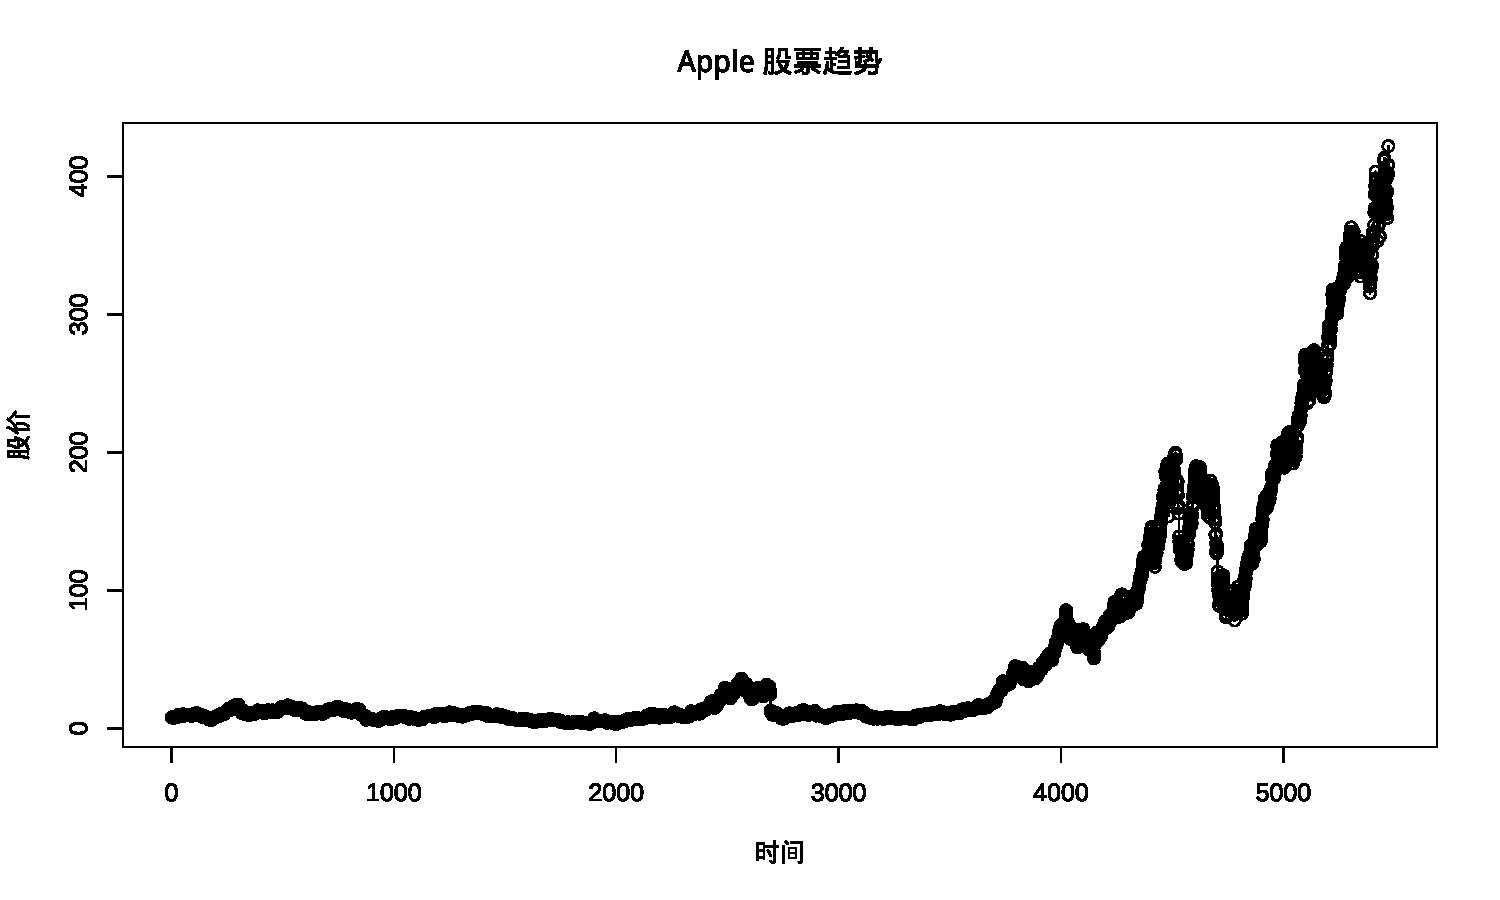
\includegraphics[width=\textwidth]{pic/Apple_stock_trend.pdf} % 插入宽度为文本宽度一半的图片
	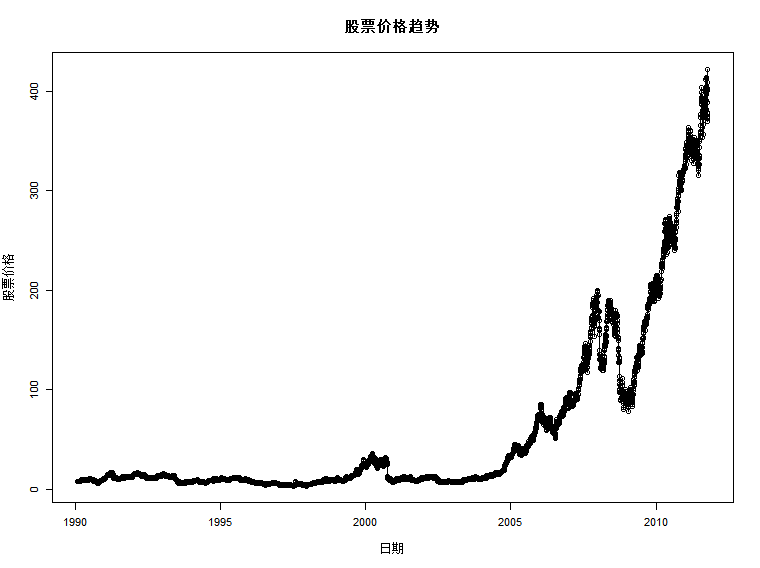
\includegraphics[width=\textwidth]{pic/stock.png}
    \caption{苹果公司股票趋势时序图} % 图片标题
	\label{} % 图片标签,用于引用
\end{figure}

早在1990年代初,苹果公司股票价格徘徊在一个相对较低的水平,大致位于100元左右。进入21世纪,苹果公司迎来了其发展历程中的转折点。随着技术创新与市场战略的成功实施,公司股票价格开始步入上升通道,至2000年前后,股价攀升至接近300元的高位。然而,在接下来的几年里,价格出现了大幅波动,有时甚至短暂回撤至200元左右。到了2005年左右,股票价格再次开始稳步上涨,并在2010年达到了一个新的高点,成功突破400元大关。然而,值得注意的是,在这期间穿插着多次短期回调与市场修正。

该时序图清晰地展现了苹果公司股票价格的长期上升趋势,这一发现暗示了序列的非平稳特性——即序列的均值随时间推移而发生显著变动,未能维持在某一恒定水平上。这一特性对于后续的时间序列分析至关重要,提示我们在进一步建模前需采取差分或其他平稳化手段以确保模型的有效性和预测精度。

\FloatBarrier

\subsection{Augmented Dickey-Fuller (ADF) 平稳性检验}

为进一步验证前述时序图中直观显示的非平稳特性,我们采用了Augmented Dickey-Fuller (ADF)检验,这是一种广泛应用的统计测试方法,用于评估时间序列的平稳性。ADF检验的核心在于检验序列是否存在单位根,从而判断其是否表现出随机游走特征。具体而言,ADF检验通过构建一个关于时间序列差分的回归模型来估计单位根的存在性,并基于回归结果计算出相应的统计量和p值,以此作为拒绝或接受原假设的依据。

\begin{lstlisting}
    adf.test(report)

    ## Warning in adf.test(report): p-value greater than printed p-value
    ##
    ## Augmented Dickey-Fuller Test
    ##
    ## data: report
    ## Dickey-Fuller = 1.5853, Lag order = 17, p-value = 0.99
    ## alternative hypothesis: stationary
\end{lstlisting}

ADF检验的结果揭示了一个重要的事实:在本案例中,序列的p值高达0.99,远超过我们设定的显著性水平(通常为0.05)。这一结果明确指示我们无法拒绝原假设,即认为该时间序列是非平稳的,存在显著的单位根效应。换句话说,序列的均值并非固定不变,而是呈现出随时间变化的趋势,这与我们在时序图中观察到的长期上升趋势相吻合。


\subsection{自相关图与偏自相关图分析}
在深入探讨时间序列的结构特征时,自相关图(Autocorrelation Function, ACF)与偏自相关图(Partial Autocorrelation Function, PACF)是不可或缺的分析工具。它们不仅能够揭示序列内部的依赖关系,还能为模型选择提供直观的指导。基于这一认识,我们对苹果公司股票价格序列进行了ACF与PACF的细致分析,以进一步探究其平稳性与潜在的自回归与移动平均特性。

接下来,我们根据自相关图和偏自相关图粗略判断序列是否平稳。若自相关图和偏自相关图里的系数很快地衰减为 0,则说明序列平稳,否则为非平稳。

\begin{lstlisting}
    # 自相关函数
    acf(as.vector(report), lag.max = 500)

    # 偏自相关函数
    pacf(as.vector(report), lag.max = 300)
\end{lstlisting}

\begin{figure}[h] % 开始一个浮动体环境,[h]指定为 here(这里)位置
	\centering % 图片居中
	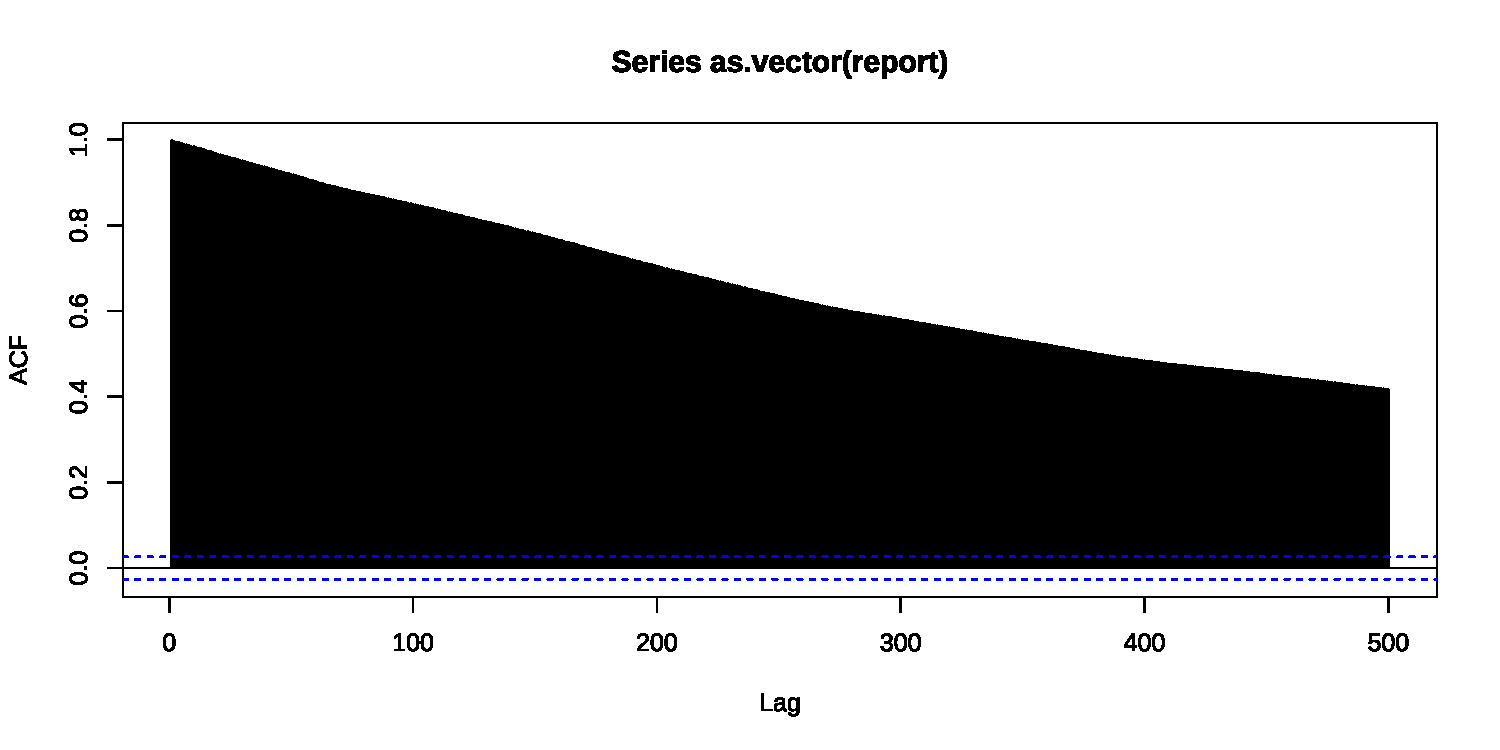
\includegraphics[width=\textwidth]{pic/acf.pdf}
    \caption{原始数据自相关图} % 图片标题
	\label{} % 图片标签,用于引用
\end{figure}

\begin{figure}[h] % 开始一个浮动体环境,[h]指定为 here(这里)位置
	\centering % 图片居中
	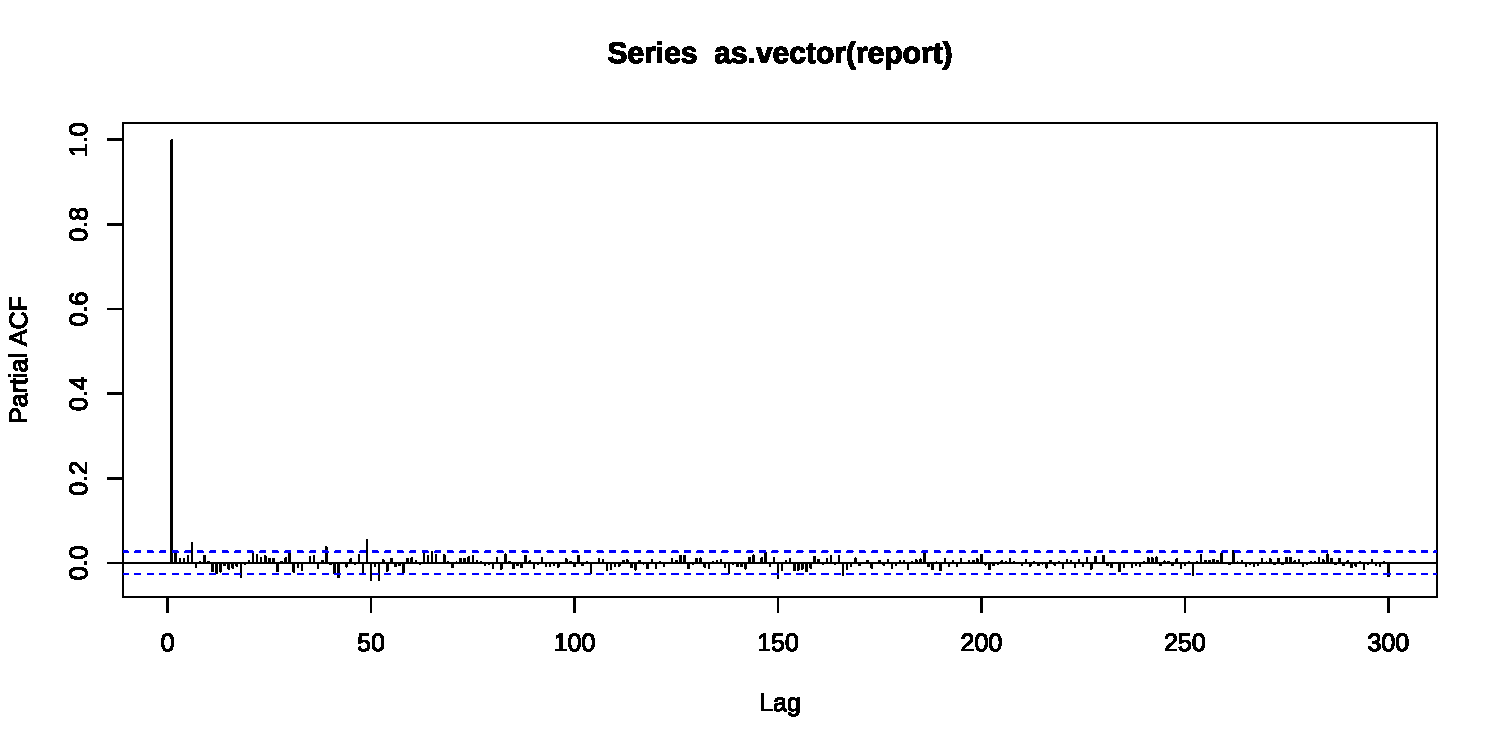
\includegraphics[width=\textwidth]{pic/pacf.pdf}
    \caption{原始数据偏自相关图} % 图片标题
	\label{} % 图片标签,用于引用
\end{figure}

\FloatBarrier

通过仔细观察自相关图与偏自相关图,我们发现苹果公司股票价格序列展现出显著的非平稳性特征。具体而言,自相关图中的系数并未迅速衰减至零,反而呈现出较为持久的拖尾现象,这与理论上平稳序列的自相关系数在零附近徘徊的行为形成鲜明对比。同样,偏自相关图亦未显示出迅速收敛的迹象,进一步证实了序列的非平稳性质。此外,自相关图中部分系数超过了置信区间(通常以两倍标准误差表示,即图中蓝色虚线),这强烈暗示序列中存在显著的自相关性,而非随机白噪声。

综合以上分析,我们可以确信苹果公司股票价格序列在未经任何预处理的情况下是非平稳的。


\section{平稳化处理}

若序列为非平稳,则需将序列通过差分转化为平稳序列。差分可以消除序列的线性趋势以及周期性。

\subsection{一阶差分消除趋势}

\begin{lstlisting}
    # 一阶差分,消除整体上升趋势
    plot(diff(report, 1), ylab = '1st Diff. of report', xlab = 'day', type = 'o')
\end{lstlisting}

画出一阶差分序列的时序图,观察序列是否平稳。利用 acf()函数。画出一阶差分序列的自相关图,通过自相关图判断序列是否平稳。

\begin{figure}[h] % 开始一个浮动体环境,[h]指定为 here(这里)位置
	\centering % 图片居中
	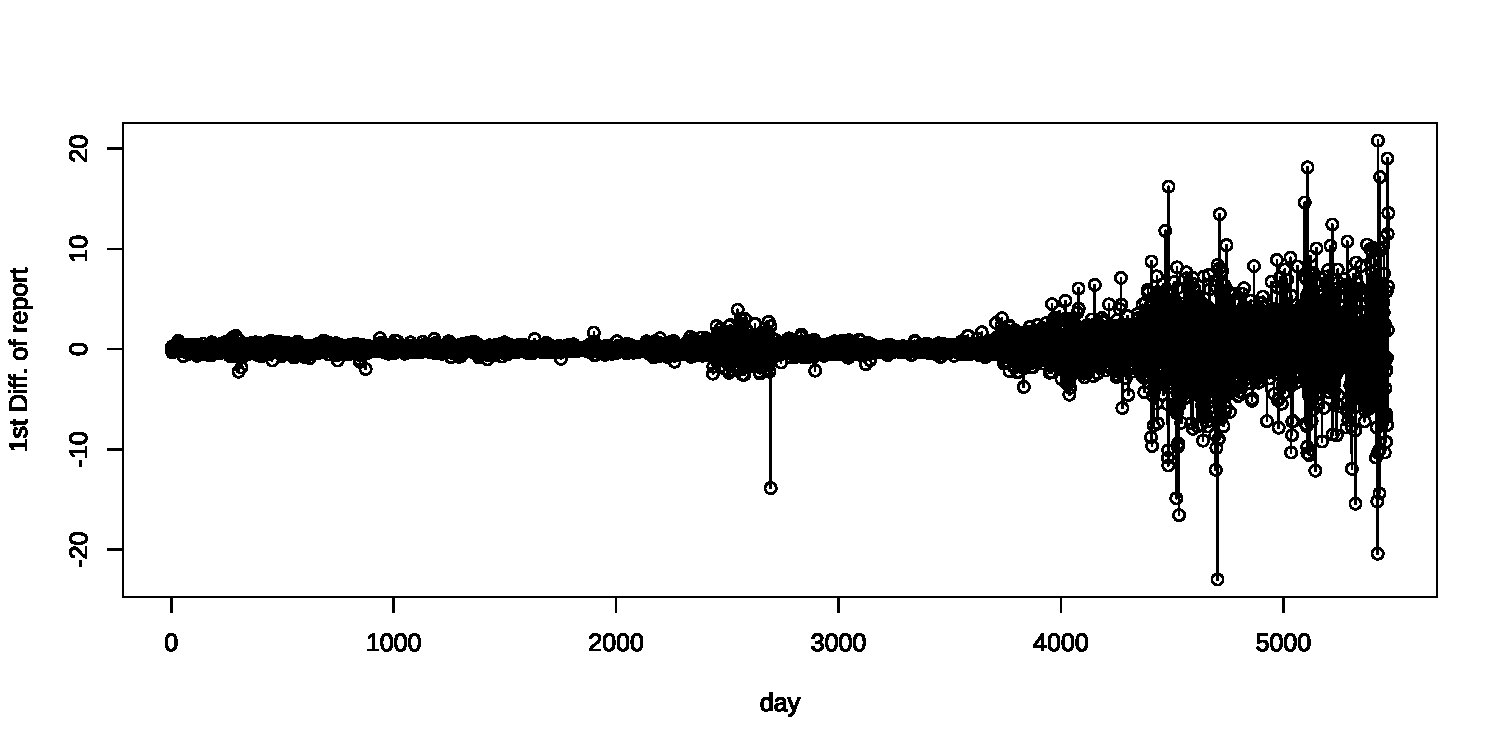
\includegraphics[width=\textwidth]{pic/1dif.pdf} % 插入宽度为文本宽度一半的图片
	\caption{一阶差分时序图} % 图片标题
	\label{} % 图片标签,用于引用
\end{figure}
\FloatBarrier

\subsection{一阶差分自相关图}
\begin{lstlisting}
    acf(as.vector(diff(report,1)),lag.max = 36)
\end{lstlisting}

\begin{figure}[h] % 开始一个浮动体环境,[h]指定为 here(这里)位置
	\centering % 图片居中
	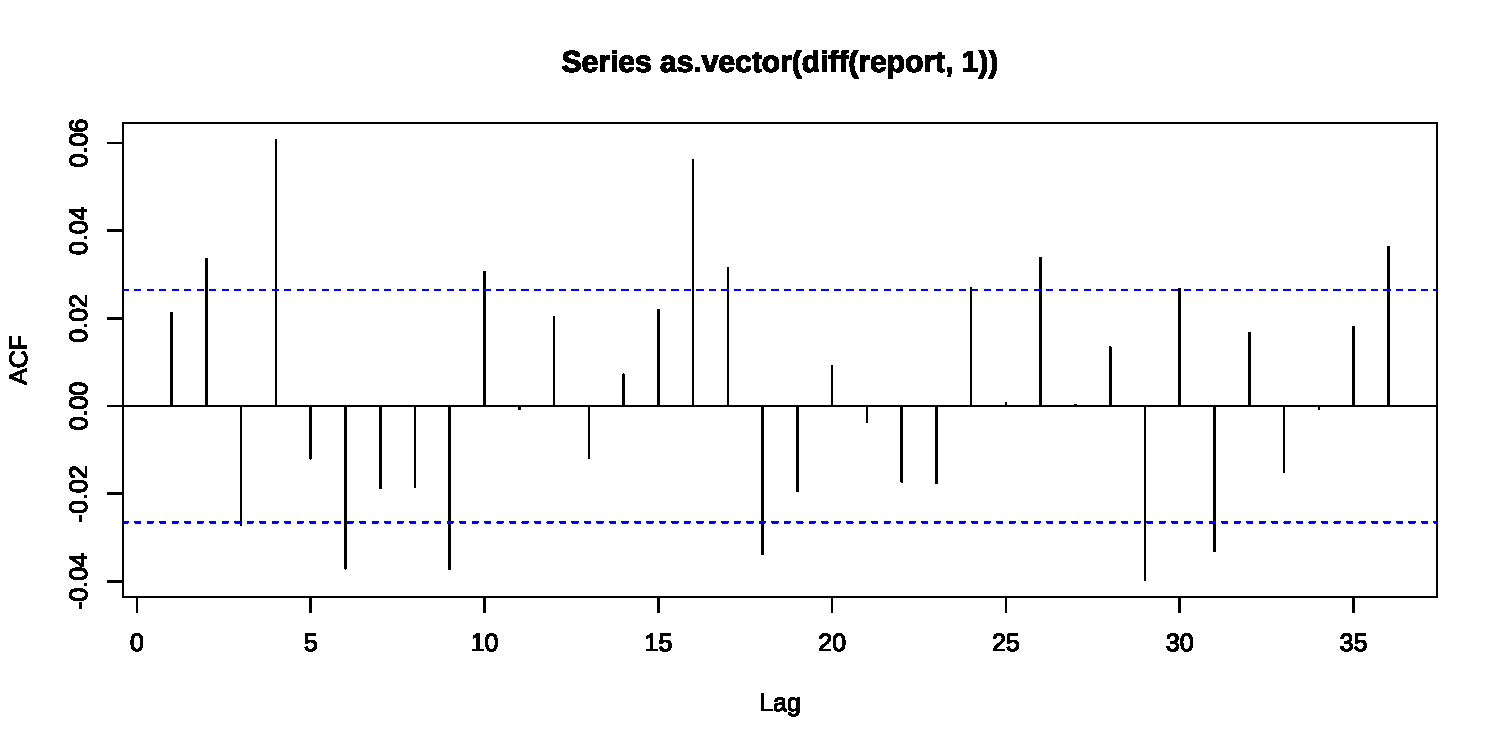
\includegraphics[width=\textwidth]{pic/acf1dif.pdf} % 插入宽度为文本宽度一半的图片
	\caption{一阶差分自相关图} % 图片标题
	\label{} % 图片标签,用于引用
\end{figure}
\FloatBarrier

\subsection{一阶差分偏自相关图}
\begin{lstlisting}
    # 一阶差分偏自相关图
    pacf(as.vector(diff(report,1)),lag.max = 36)
\end{lstlisting}

\begin{figure}[h] % 开始一个浮动体环境,[h]指定为 here(这里)位置
	\centering % 图片居中
	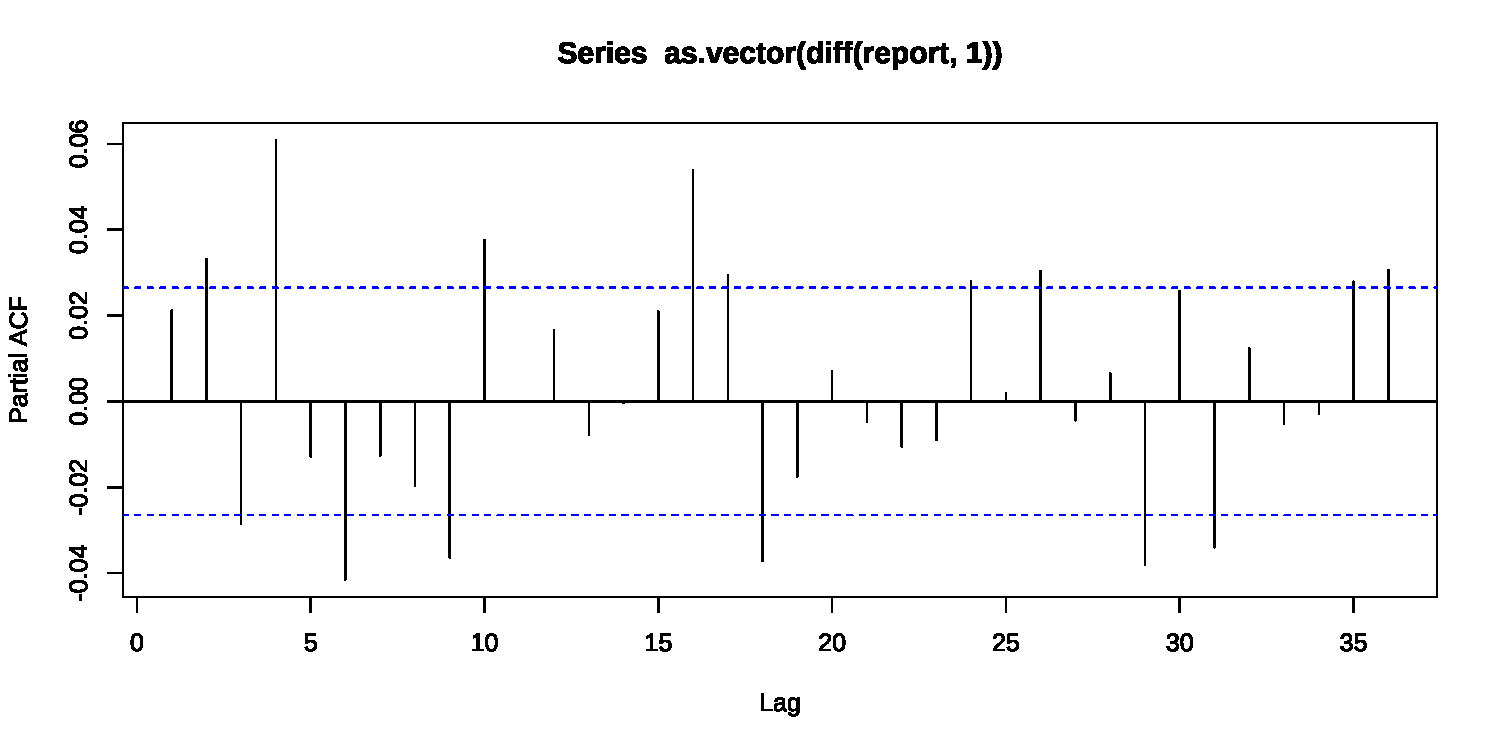
\includegraphics[width=\textwidth]{pic/pacf1dif.pdf} % 插入宽度为文本宽度一半的图片
	\caption{一阶差分偏自相关图} % 图片标题
	\label{} % 图片标签,用于引用
\end{figure}
\FloatBarrier
从时序图可得出数据不存在明显的周期性。自相关图中系数没有快速的减为 0,故判断该序列为非平稳序列。

\subsection{一阶差分 ADF 平稳性检验}
为使以上结论更具说服力故调用 adf.test()函数,观察序列是否平稳。

\begin{lstlisting}
    # 一阶差分 adf 平稳性检验
    adf.test(diff(report,1))
    ## Warning in adf.test(diff(report, 1)): p-value smaller than printed p-value
    ##
    ## Augmented Dickey-Fuller Test
    ##
    ## data: diff(report, 1)
    ## Dickey-Fuller = -16.532, Lag order = 17, p-value = 0.01
    ## alternative hypothesis: stationary
\end{lstlisting}

p-value 小于 0.05,拒绝原假设,即该时间序列为平稳序列。

\subsection{利用EACF确定ARIMA模型阶数}

Extended Autocorrelation Function (EACF) 成为了我们识别合适ARIMA模型阶数的有力工具。EACF方法,以其独特的矩阵形式,为我们提供了直观的视觉辅助,帮助判断模型中自回归(AR)与移动平均(MA)部分的最优阶数。基于这一理念,我们对苹果公司股票价格序列的一阶差分进行了EACF分析,以期找到最能贴合数据特性的模型配置。

\begin{lstlisting}
    eacf(as.vector(diff(report,1)),ar.max=6,ma.max=5)

\end{lstlisting}
\begin{table}[h]
    \centering
    \begin{tabular}{|c|c|c|c|c|c|c|}
    \hline
    AR/MA & 0 & 1 & 2 & 3 & 4 & 5 \\
    \hline
    0 & o & x & x & x & o & x \\
    \hline
    1 & x & x & \cellcolor{yellow}\textcolor{red}{o} & x & o & o \\
    \hline
    2 & x & x & \cellcolor{yellow}\textcolor{red}{o} & x & x & x \\
    \hline
    3 & x & x & x & x & x & o \\
    \hline
    4 & x & x & x & x & x & o \\
    \hline
    5 & x & x & x & x & x & o \\
    \hline
    6 & x & x & x & x & x & x \\
    \hline
    \end{tabular}
    \caption{AR/MA关系表}
    \label{tab:ar-ma-relations}
\end{table}

细观EACF图,我们注意到ARIMA模型的潜在阶数组合。具体而言,表中“o”标记表示模型在该阶数上的可能性较大,而“x”则暗示了相应阶数的不适用性。通过分析,我们发现当AR阶数为1或2,MA阶数为2时,模型表现出了较好的拟合度,这意味着序列可能遵循\(\text{ARIMA}(1,0,2)\)或\(\text{ARIMA}(2,0,2)\)的模型结构。

此外,由于我们已知序列在差分后表现为平稳,此处的差分阶数应调整为1,以反映序列的实际特性,因此最终模型应考虑为\(\text{ARIMA}(1,1,2)\)或\(\text{ARIMA}(2,1,2)\)。

\section{建立模型}

为了进一步确定模型是\(\text{ARIMA}(1,1,2)\)和\(\text{ARIMA}(2,1,2)\)中的哪一个,我们比较了一系列统计指标加以确定。

\subsection{模型拟合}

利用 ARIMA 函数进行 ARIMA(1,0,2)拟合
\begin{lstlisting}
    ar1_model <- auto.arima(diff(report), max.order = 2, seasonal = FALSE, stationary = TRUE, ic = "aic")
    summary(ar1_model)
    ## Series: diff(report) 
    ## ARIMA(1,0,2) with non-zero mean 
    ## 
    ## Coefficients:
    ##           ar1     ma1     ma2    mean
    ##       -0.7827  0.8069  0.0562  0.0738
    ## s.e.   0.1405  0.1400  0.0157  0.0294
    ## 
    ## sigma^2 = 4.347:  log likelihood = -11780.49
    ## AIC=23570.98   AICc=23570.99   BIC=23604.02
    ## 
    ## Training set error measures:
    ##                       ME     RMSE       MAE  MPE MAPE      MASE          ACF1
    ## Training set 0.001952685 2.084067 0.9756905 -Inf  Inf 0.7126346 -0.0004015358
\end{lstlisting}

% 输出给出了模型的系数和标准误差。具体来说,自回归项的系数为0.0214,截距(intercept)的系数为0.0757。它们的标准误差(s.e.)分别为0.0136和0.0288,较小的误差说明了模型拟合得很好。模型的方差估计为4.359,对数似然为-11790.47。这些指标可以用来评估模型的拟合程度,越小的方差和更高的对数似然通常表示模型拟合得更好。AIC可以用于比较不同模型之间的拟合优度,这里输出提供了AIC(赤池信息准则)的值,为23584.94。

\begin{lstlisting}
    m010_report<- arima(diff(report), order=c(1, 0, 2), method='ML')
    print(m010_report)
    ## 
    ## Call:
    ## arima(x = diff(report), order = c(1, 0, 2), method = "ML")
    ## 
    ## Coefficients:
    ##           ar1     ma1     ma2  intercept
    ##       -0.7840  0.8082  0.0562     0.0753
    ## s.e.   0.1397  0.1392  0.0157     0.0294
    ## 
    ## sigma^2 estimated as 4.343:  log likelihood = -11780.49,  aic = 23568.98
\end{lstlisting}

\begin{table}[H]
    \centering
    \begin{tabular}{lcccc} % l 表示左对齐的列,c 表示居中对齐的列
    \toprule % 顶部的加粗横线
    & ar1 & ma1 & ma2 & intercept \\
    \midrule % 分割线,比\toprule和\bottomrule细
    参数估计 & -0.7840 & 0.8082 & 0.0562 & 0.0753 \\
    参数标准误差 & 0.1397 & 0.1392 & 0.0157 & 0.0294 \\
    \bottomrule % 底部的加粗横线
    \end{tabular}
    \caption{ARIMA(1,0,2)模型参数估计及其标准误差}
    \label{tab:arima-param-estimates-transposed}
\end{table}

\begin{table}[H]
    \centering
    \begin{tabular}{lccc} % l 表示左对齐的列,c 表示居中对齐的列
    \toprule % 顶部的加粗横线
    & $\sigma^2$ 估计 & 对数似然 & AIC \\
    \midrule % 分割线,比\toprule和\bottomrule细
    值 & 4.343 & -11780.49 & 23568.98 \\
    \bottomrule % 底部的加粗横线
    \end{tabular}
    \caption{ARIMA(1,0,2)统计量值}
    \label{tab:statistics-values-transposed}
\end{table}

\begin{table}[H]
    \centering
    \begin{tabular}{lccccc} % l 表示左对齐的列,c 表示居中对齐的列
    \toprule % 顶部的加粗横线
    & ar1 & ar2 & ma1 & ma2 & intercept \\
    \midrule % 分割线,比\toprule和\bottomrule细
    参数估计 & -0.4852 & 0.4485 & 0.5068 & -0.4038 & 0.0754 \\
    参数标准误差 & 0.2191 & 0.2178 & 0.2244 & 0.2217 & 0.0300 \\
    \bottomrule % 底部的加粗横线
    \end{tabular}
    \caption{ARIMA(2,0,2)模型参数估计及其标准误差}
    \label{tab:arima-parameters-transposed}
\end{table}

\begin{table}[H]
    \centering
    \begin{tabular}{lccc} % l 表示左对齐的列,c 表示居中对齐的列
    \toprule % 顶部的加粗横线
    & $\sigma^2$ 估计 & 对数似然 & AIC \\
    \midrule % 分割线,比\toprule和\bottomrule细
    值 & 4.343 & -11780.16 & 23570.32 \\
    \bottomrule % 底部的加粗横线
    \end{tabular}
    \caption{ARIMA(2,0,2)统计量值}
    \label{tab:statistics-transposed}
\end{table}

下面针对这两个拟合之后的结果进行比较。

首先看参数估计的标准误差,较小的标准误差通常意味着更精确的参数估计。因此由图中可以看出ARIMA(1,0,2)的参数标准误差普遍小于ARIMA(2,0,2)的误差。同时这两个模型的方差估计值,即残差项的方差均为4.343这一数据说明,观测值与模型预测值之间的差异都比较小。我们再来看两者对数似然值的比较,对数似然值描述了给定模型下观测数据出现的概率。因此对于对数似然值而言,越大越好。从表格中我们看到ARIMA(1,0,2)模型的对数似然值为-11780.49,而ARIMA(2,0,2)模型的对数似然值为-11780.16。因此,在这一指标上,ARIMA(2,0,2)模型略优于ARIMA(1,0,2)模型。最后从AIC值分析,ARIMA(1,0,2)模型的AIC值为23568.98,而ARIMA(2,0,2)模型的AIC值为23570.32。由于AIC值越小越好,因此ARIMA(1,0,2)模型在AIC值上的表现也好于ARIMA(2,0,2)模型。


\subsection{参数的显著性检验}
参数的显著性检验:用估计出的系数除以其的标准差(s.e.)得到的商与 T 统计量 5\%临界值 1.96 比较,商的绝对值大于 1.96,则拒绝原假设,认为系数显著的不为 0,否则认为系数不显著。系数不显著的可以去掉。

\[ t_{统计量(ar1)} = \frac{-0.7827}{0.1405} \approx -5.57,\text{显著} \]

\[ t_{统计量(ma1)} = \frac{0.8069}{0.1400} \approx 5.76,\text{显著} \]

\[ t_{统计量(ma2)} = \frac{0.0562}{0.0157} \approx 3.58,\text{显著} \]

\subsection{残差的正态性检验}
画出残差的 QQ 图即可判断,QQ 图中残差基本完全落在 45°线上即为符合正态性假设。否则模型可能出现错误。

\begin{lstlisting}
    qqnorm(m121.report$residuals,main='Q-Q 图')
    qqline(m121.report$residuals)
\end{lstlisting}

\begin{figure}[H]
    \begin{minipage}[t]{0.5\linewidth}
    \centering
    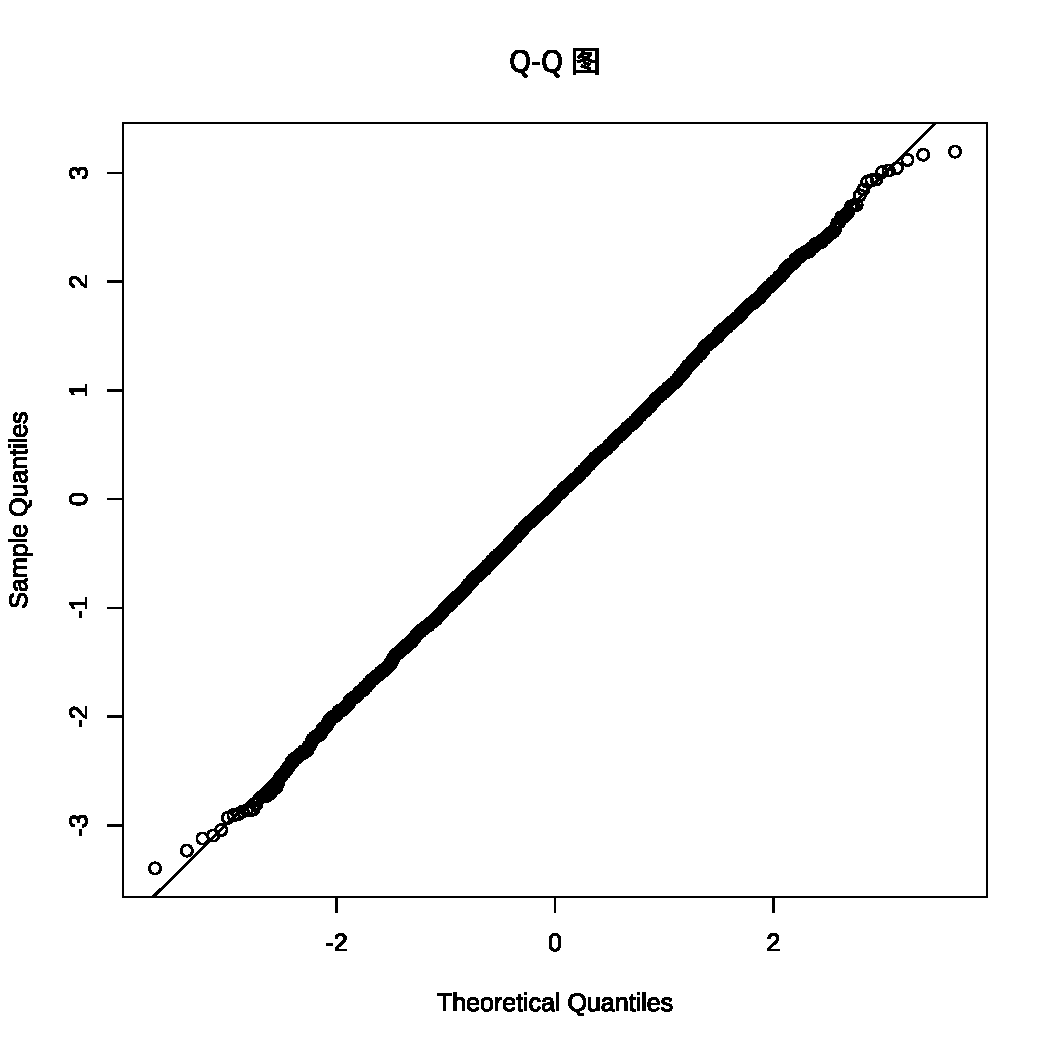
\includegraphics[width=2.2in]{pic/qq_fake.pdf}
    \caption{ARIMA(1,0,2) Q-Q图}
    \label{fig:side:a}
    \end{minipage}%
    \begin{minipage}[t]{0.5\linewidth}
    \centering
    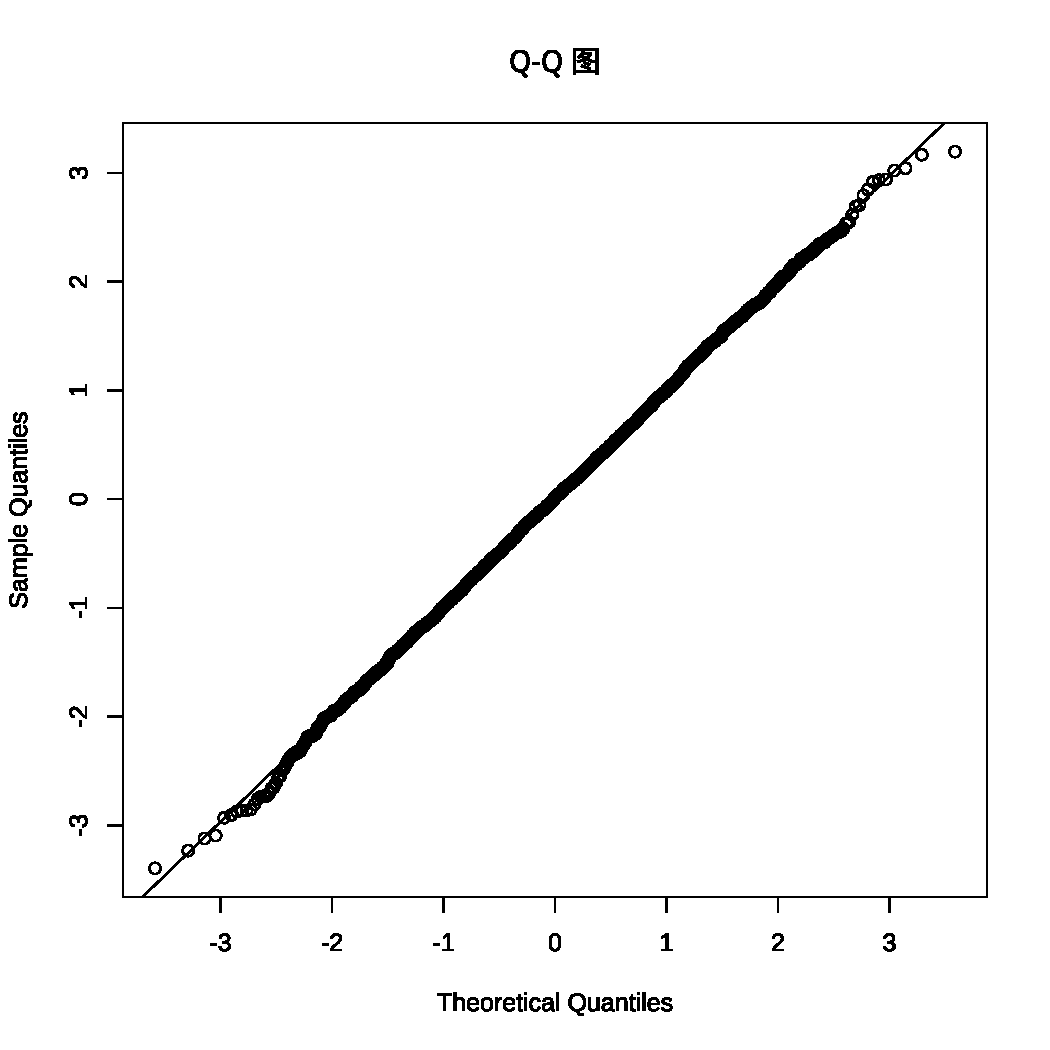
\includegraphics[width=2.2in]{pic/qq_fake1.pdf}
    \caption{ARIMA(2,0,2) Q-Q图}
    \label{fig:side:b}
    \end{minipage}
\end{figure}

\subsection{残差的自相关函数图和偏自相关函数图}
\begin{lstlisting}
    # 计算 ARIMA(1, 0, 2) 模型的残差
    residuals <- resid(m010_report)
    
    # 绘制残差的自相关函数图
    acf(residuals, lag.max = 36)
\end{lstlisting}

\begin{figure}[H] % 开始一个浮动体环境,[h]指定为 here(这里)位置
	\centering % 图片居中
	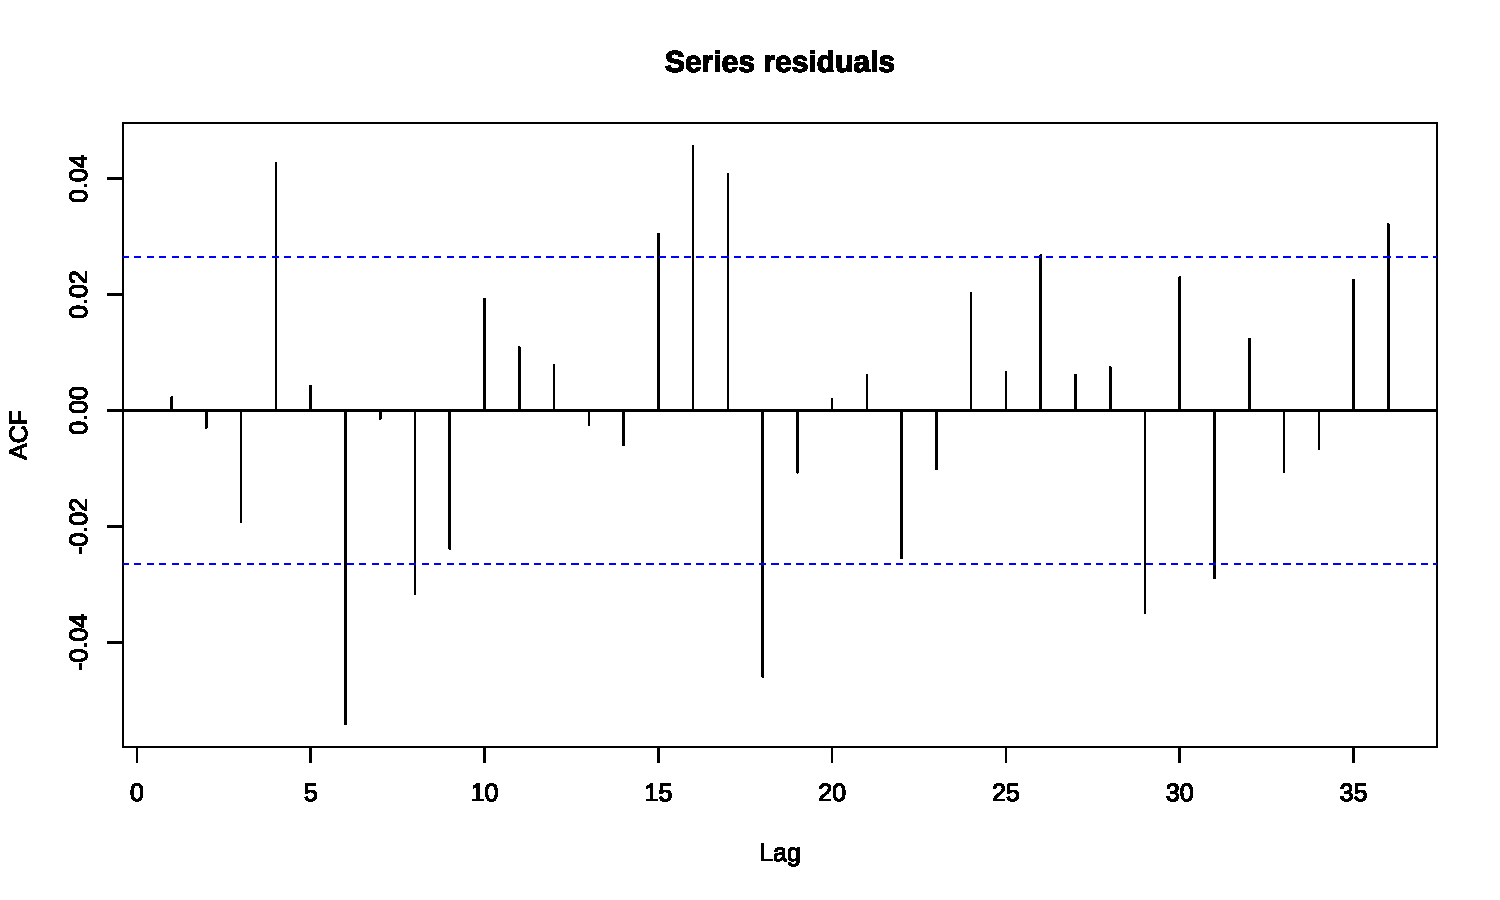
\includegraphics[width=0.75\textwidth]{pic/resacf.pdf} % 插入宽度为文本宽度一半的图片
	\caption{残差的自相关函数图} % 图片标题
\end{figure}

\begin{lstlisting}
    # 一阶差分偏自相关图
    pacf(residuals, lag.max = 36)
\end{lstlisting}

\begin{figure}[H] % 开始一个浮动体环境,[h]指定为 here(这里)位置
	\centering % 图片居中
	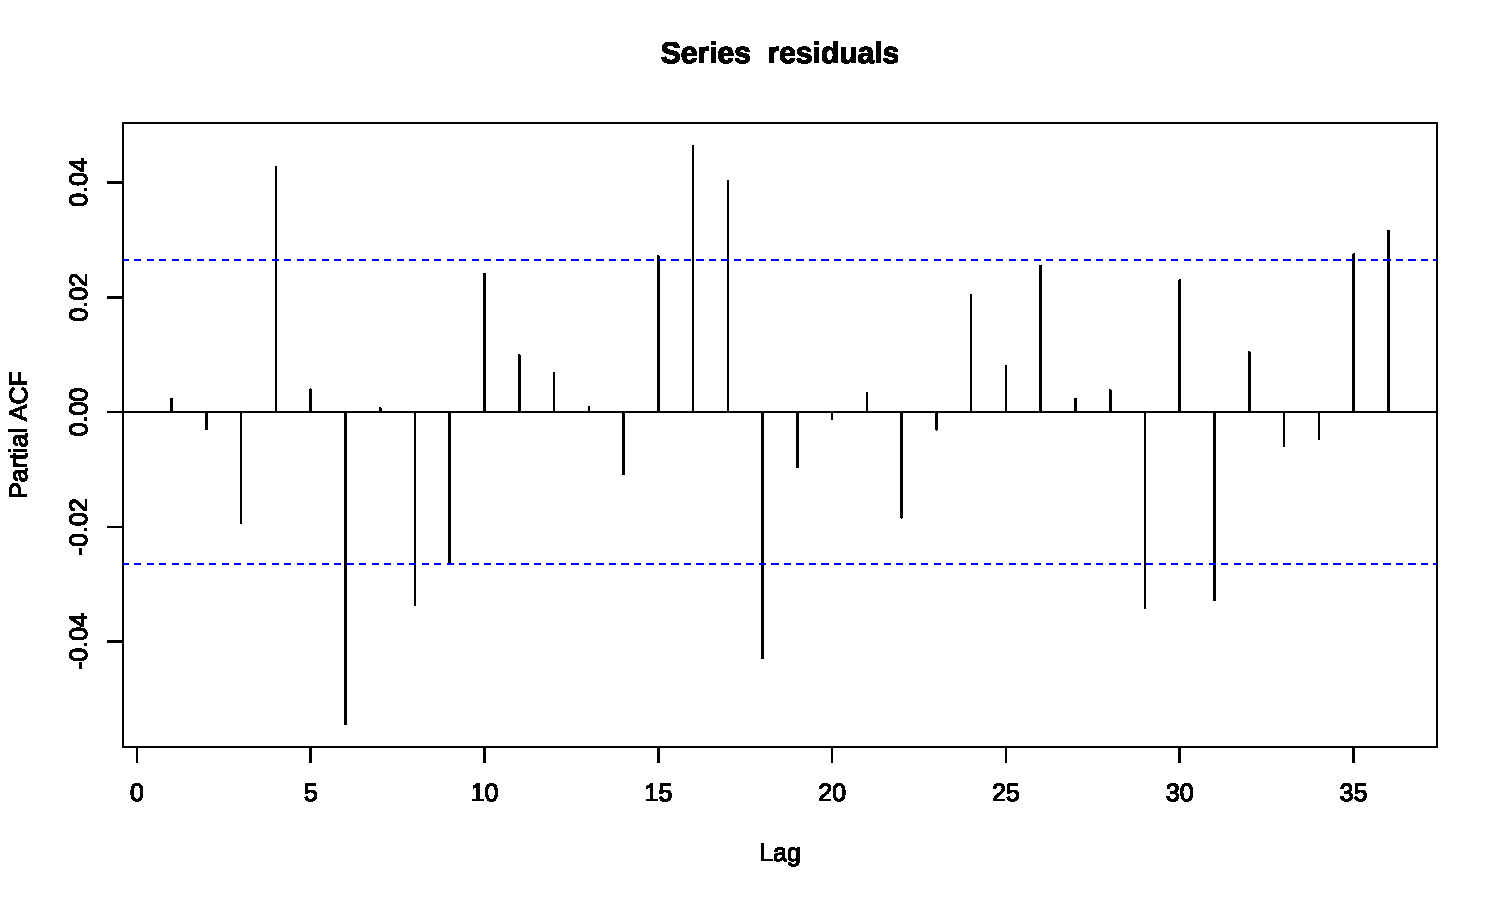
\includegraphics[width=0.75\textwidth]{pic/respacf.pdf} % 插入宽度为文本宽度一半的图片
	\caption{残差的偏自相关函数图} % 图片标题
\end{figure}

做出两个模型的ACF和PACF图发现,两个模型的ACF和PACF均呈拖尾。


\subsection{残差的白噪声检验}
白噪声检验作为模型残差分析的核心组成部分,其重要性不言而喻。白噪声序列,定义为一系列独立同分布的随机变量,其均值为零,方差保持恒定,且任意两个不同时间点上的变量之间不存在相关性。在时间序列分析的语境下,当模型残差被证明遵循白噪声分布时,这标志着序列中所有可预测的、系统性的信息已被模型充分提取,剩余的仅是随机扰动,即那些无法通过现有模型结构捕捉的不确定性成分。

利用 Ljung-Box 对一阶差分序列的残差进行白噪声检验。如果 \(p<0.05\),拒绝原假设,说明原始序列存在相关性;如果 \(p \geq 0.05\),接受原假设,说明原始序列独立,纯随机,残差是白噪声。
\begin{lstlisting}
    Box.test(m010_report$residuals,type="Ljung-Box")
    ##  Box-Ljung test
    ## data:  m010_report$residuals
    ## X-squared = 0.00087885, df = 1, p-value = 0.9763
\end{lstlisting}

\begin{table}[H]
    \centering
    \begin{tabular}{ll} % l 表示左对齐的列
    \toprule % 顶部的加粗横线
    模型 & p-value \\
    \midrule % 分割线,比\toprule和\bottomrule细
    ARIMA(1,0,2) & 0.9763 \\
    ARIMA(2,0,2) & 0.8676 \\
    \bottomrule % 底部的加粗横线
    \end{tabular}
    \caption{ARIMA模型的p-value}
    \label{tab:model-pvalues}
\end{table}

两个模型的 p-value 分别为 0.9763 和 0.8676,大于 0.05,因此序列的残差为白噪声,原始序列独立,纯随机。

综合以上分析,我们可以得出结论:ARIMA(1,0,2)相对于ARIMA(2,0,2)在对数似然函数值和AIC准则下表现更好,说明它能够更好地拟合训练数据,并且前者在模型复杂度更低的情况下取得了更好的表现。因此,在这两个模型中,第一个模型更具有解释力和预测能力。故选择第一个模型进行最后的预测。



% p-value 为 0.9583,大于 0.05,因此该序列的残差为白噪声,原始序列独立,纯随机。

\section{模型预测}

利用最终确定的ARIMA模型,我们对未来一年内的苹果公司股票价格进行了预测,绘制了预测图,为市场参与者提供了有价值的参考信息。此研究不仅增强了我们对苹果股票动态的洞察力,也展现了时间序列分析在预测金融市场的实用性与潜力。

本次研究之旅,我们秉持着严谨的学术态度与系统化的分析方法,深入探索了苹果公司股票价格波动的本质,揭示了其背后隐含的复杂动态与规律性。借助于时间序列分析这一强大工具,我们不仅捕捉到了苹果公司股票价格随时间演进的细微脉络,还构建了一套精确的预测模型,旨在为投资者提供前瞻性的市场洞见。尤为重要的是,我们通过对残差序列的细致检验,确保了模型的稳健性与可靠性,为后续的市场预测创造了更加全面的视角。

\begin{lstlisting}
    fit =stats::arima(report,order=c(1,1,2))
    plot(forecast(fit,365))
\end{lstlisting}

\begin{figure}[H] % 开始一个浮动体环境,[h]指定为 here(这里)位置
	\centering % 图片居中
	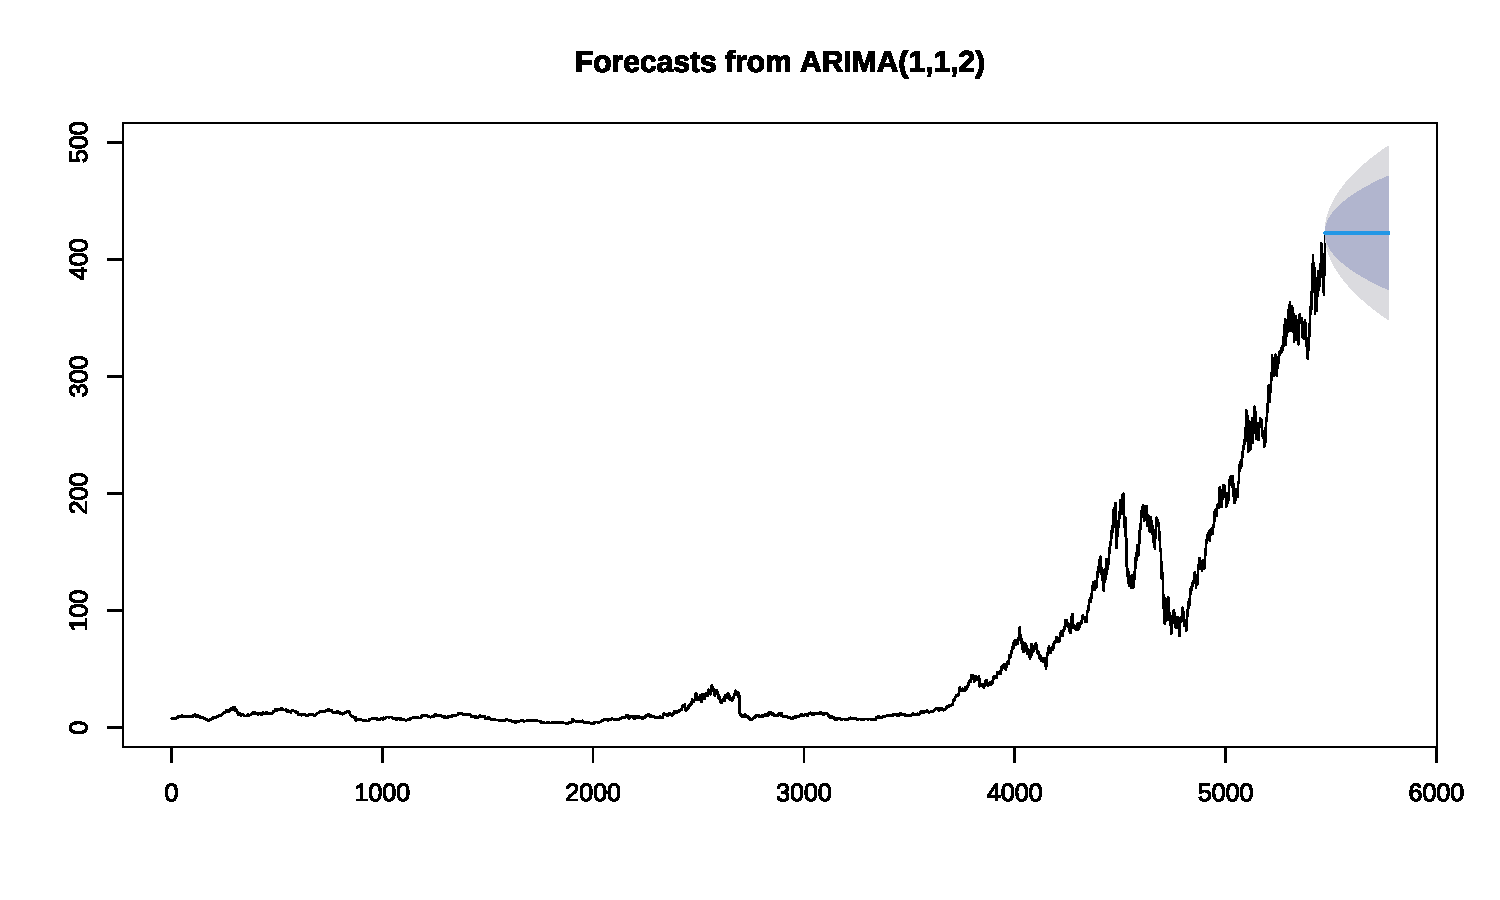
\includegraphics[width=\textwidth]{pic/forecast.pdf} % 插入宽度为文本宽度一半的图片
	\caption{模型预测图} % 图片标题
	\label{} % 图片标签,用于引用
\end{figure}
\FloatBarrier


\end{document}